% !TEX program = xelatex
% 实验二 实验报告骨架：结构、图表与版式已就位，正文段落请自己撰写（任务书要求报告不得使用大模型辅助）
\documentclass[UTF8,a4paper,12pt]{ctexart}
\usepackage[margin=2.2cm]{geometry}
\usepackage{graphicx}
\usepackage{booktabs}
\usepackage{array}
\usepackage{longtable}
\usepackage{caption}
\usepackage{subcaption}
\usepackage{float}
\usepackage{enumitem}
\usepackage{xcolor}
\usepackage{hyperref}
\hypersetup{colorlinks=true,linkcolor=black,urlcolor=blue}
\setlist{nosep,leftmargin=2.2em}
\captionsetup{font=small,labelsep=quad}
\graphicspath{{UML/}{UI界面/}}

% 占位标记：写完后把这些命令删掉
\newcommand{\todo}[1]{\par\vspace{2pt}{\color{gray}\small 〔待写〕#1}\par\vspace{2pt}}

\title{\bfseries 二手交易系统的软件设计与建模}
\author{王彦君\quad 241220143}
\date{2026 年 11 月}

\pagestyle{plain}
\begin{document}
\maketitle

\begin{center}
\begin{tabular}{ll}
课程：软件工程 & 实验：实验二 软件设计与建模 \\
学号：241220143 & 姓名：王彦君 \\
项目：校园二手交易系统 & 需求来源：实验一需求分析（REQ-001～REQ-035） \\
\end{tabular}
\end{center}

\vspace{0.6em}
\noindent\textbf{说明}：本报告由 5 章组成，对应任务书的三项必含内容与"大模型使用"专章。
全部 UML 图由 PlantUML 源码（\texttt{UML/*.puml}）渲染，界面稿见 \texttt{UI界面/}。

\tableofcontents
\newpage

%=====================================================================
\section{软件的主要功能}

\subsection{项目说明}
\todo{说明所选项目：校园二手交易，解决"口头订下、先后无记录、交易不可追溯"的问题；明确不实现支付/物流/在线聊天/议价。约 150 字。}

\subsection{主要功能}
\todo{6 条功能，每条一句话：商品发布与审核、分类维护、多条件查询与统计、预约与候补、交易确认与双向评价、操作日志。}

\subsection{功能模块划分}
\todo{引出表 \ref{tab:modules}：7 个模块与实验一需求的对应关系，并说明"每条需求都能追到唯一模块"。}

\begin{table}[H]
\centering\small
\caption{功能模块与需求对应（对应实验一的七个业务模块）}\label{tab:modules}
\begin{tabular}{p{1.1cm}p{3.3cm}p{8.6cm}}
\toprule
编号 & 模块 & 覆盖需求 \\
\midrule
M1 & 账号与权限 & REQ-001、002、019、031、032、033 \\
M2 & 商品与审核 & REQ-003、004、005、006、007、022、027 \\
M3 & 分类 & REQ-028、029 \\
M4 & 查询与统计 & REQ-008、016、018 \\
M5 & 预约与候补 & REQ-009、010、011、012、013、021、024、030、034、035 \\
M6 & 交易与评价 & REQ-025、026 \\
M7 & 数据与日志 & REQ-014、015、017、020、023 \\
\bottomrule
\end{tabular}
\end{table}

%=====================================================================
\section{软件架构 UML 图}

\subsection{组件图：模块划分与模块间交互}
\begin{figure}[H]
\centering
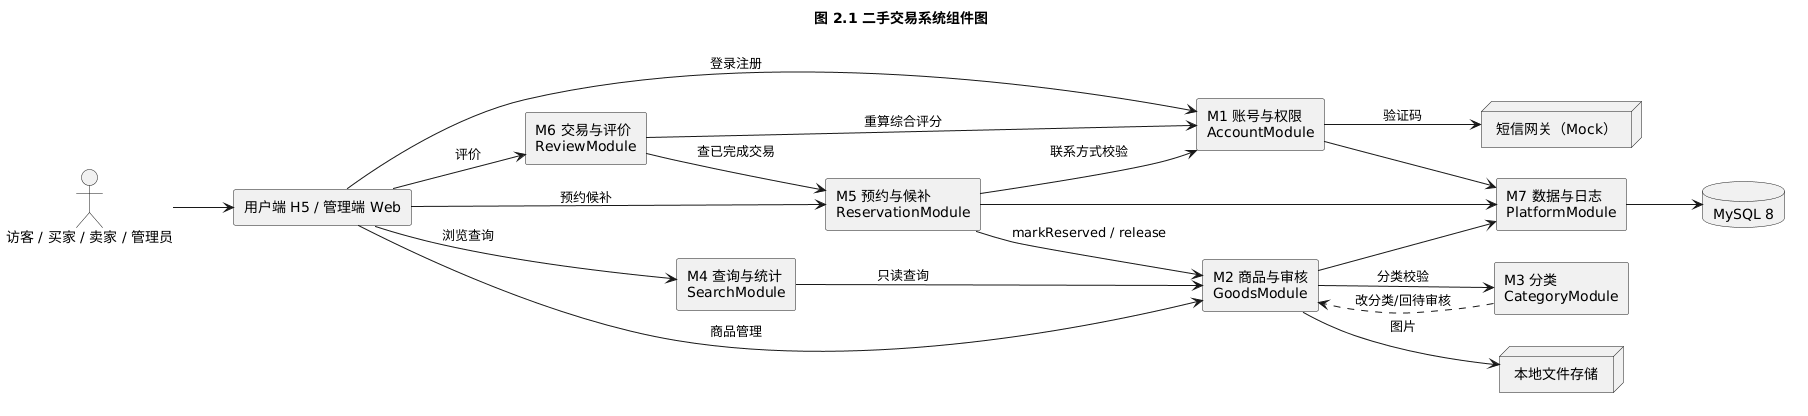
\includegraphics[width=\textwidth]{UML组件图.png}
\caption{系统组件图}\label{fig:component}
\end{figure}
\todo{读图说明 + 模块交互的 5 条关键依赖（谁调用谁、为什么），可引表 \ref{tab:deps}。}

\begin{table}[H]
\centering\small
\caption{模块之间的关键交互}\label{tab:deps}
\begin{tabular}{p{2.2cm}p{3.6cm}p{7.2cm}}
\toprule
调用方 → 被调用方 & 接口 & 这样设计的原因 \\
\midrule
M5 → M2 & \texttt{markReserved / release} & 预约状态与商品状态必须同事务变更（REQ-011、020、035） \\
M5 → M1 & \texttt{checkContactReady} & 任一方未填手机号时拒绝预约（REQ-009） \\
M2 → M7 & \texttt{log / @Transactional} & 关键操作留痕且状态变更原子（REQ-017、020） \\
M3 → M2 & \texttt{resetToPending} & 管理员改分类视同内容变更，商品回待审核（REQ-029） \\
M6 → M5 & \texttt{findCompleted} & 只有已完成交易才能评价（REQ-025） \\
\bottomrule
\end{tabular}
\end{table}

\subsection{包图：分层与目录结构}
\begin{figure}[H]
\centering
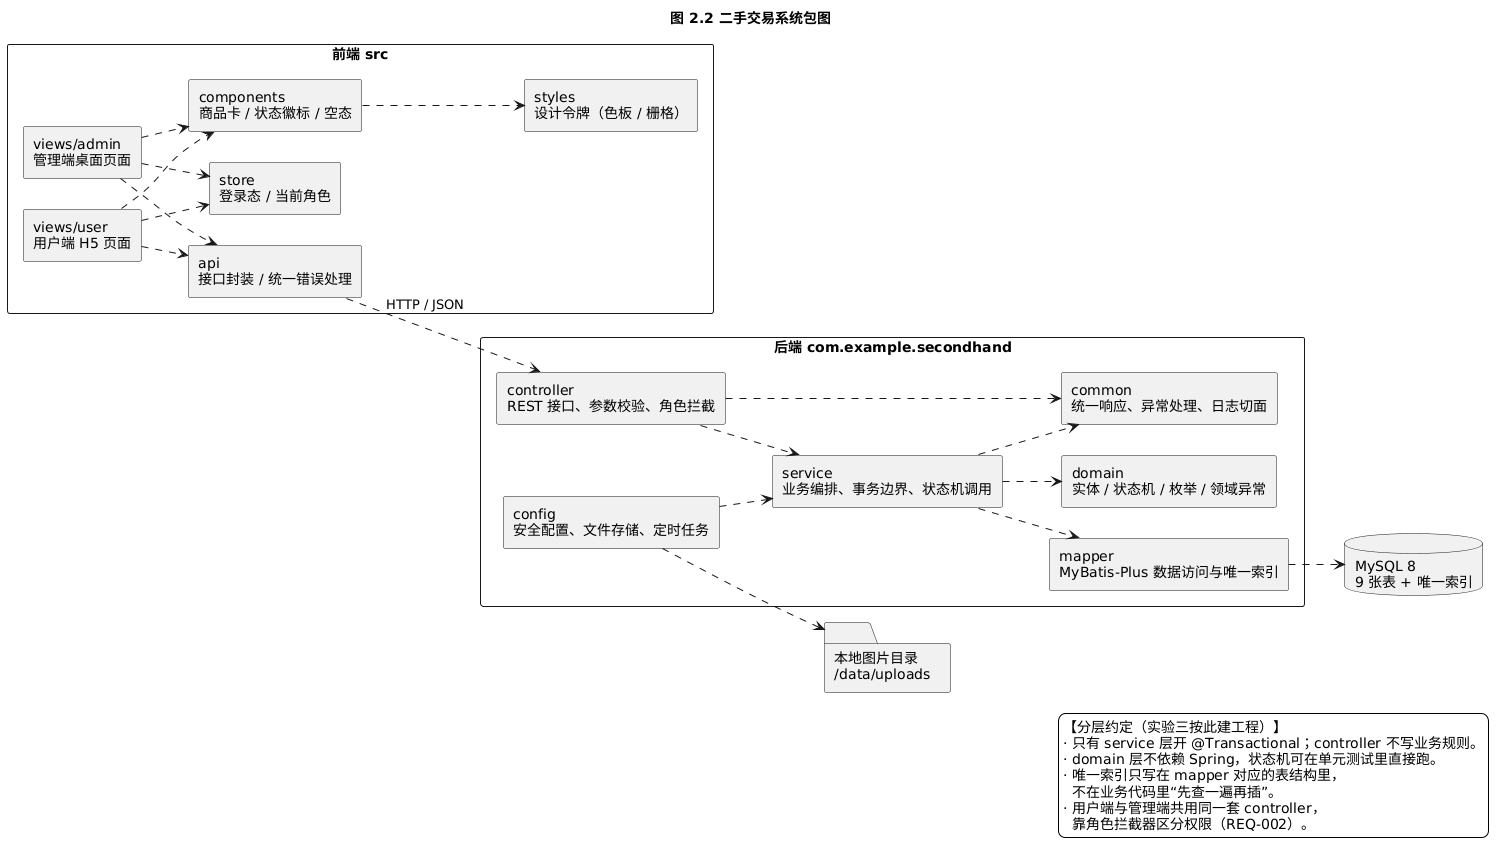
\includegraphics[width=\textwidth]{UML包图.png}
\caption{系统包图}\label{fig:package}
\end{figure}
\todo{说明为什么这样分层：只有 service 开事务、domain 不依赖框架、唯一索引只写在表结构里、两端共用 controller。}

\subsection{类图：领域实体与领域服务}
\begin{figure}[H]
\centering
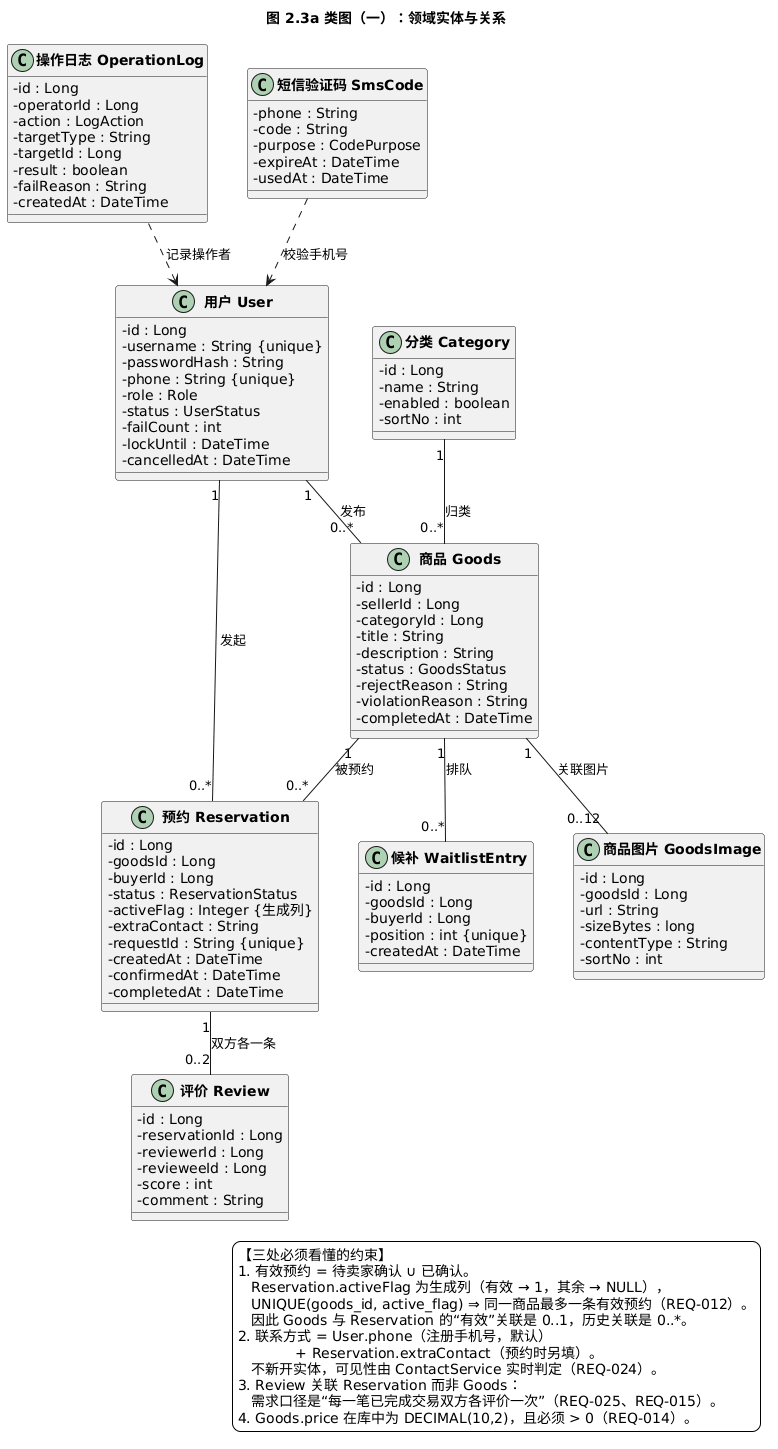
\includegraphics[width=0.66\textwidth]{UML类图-实体.png}
\caption{领域实体类图}\label{fig:class1}
\end{figure}
\todo{逐类说明职责 + 多重度；重点讲三处：\texttt{Reservation.activeFlag}（唯一有效预约）、
\texttt{User.phone + Reservation.extraContact}（联系方式不单开实体）、\texttt{Review} 关联预约而非商品。}

\begin{figure}[H]
\centering
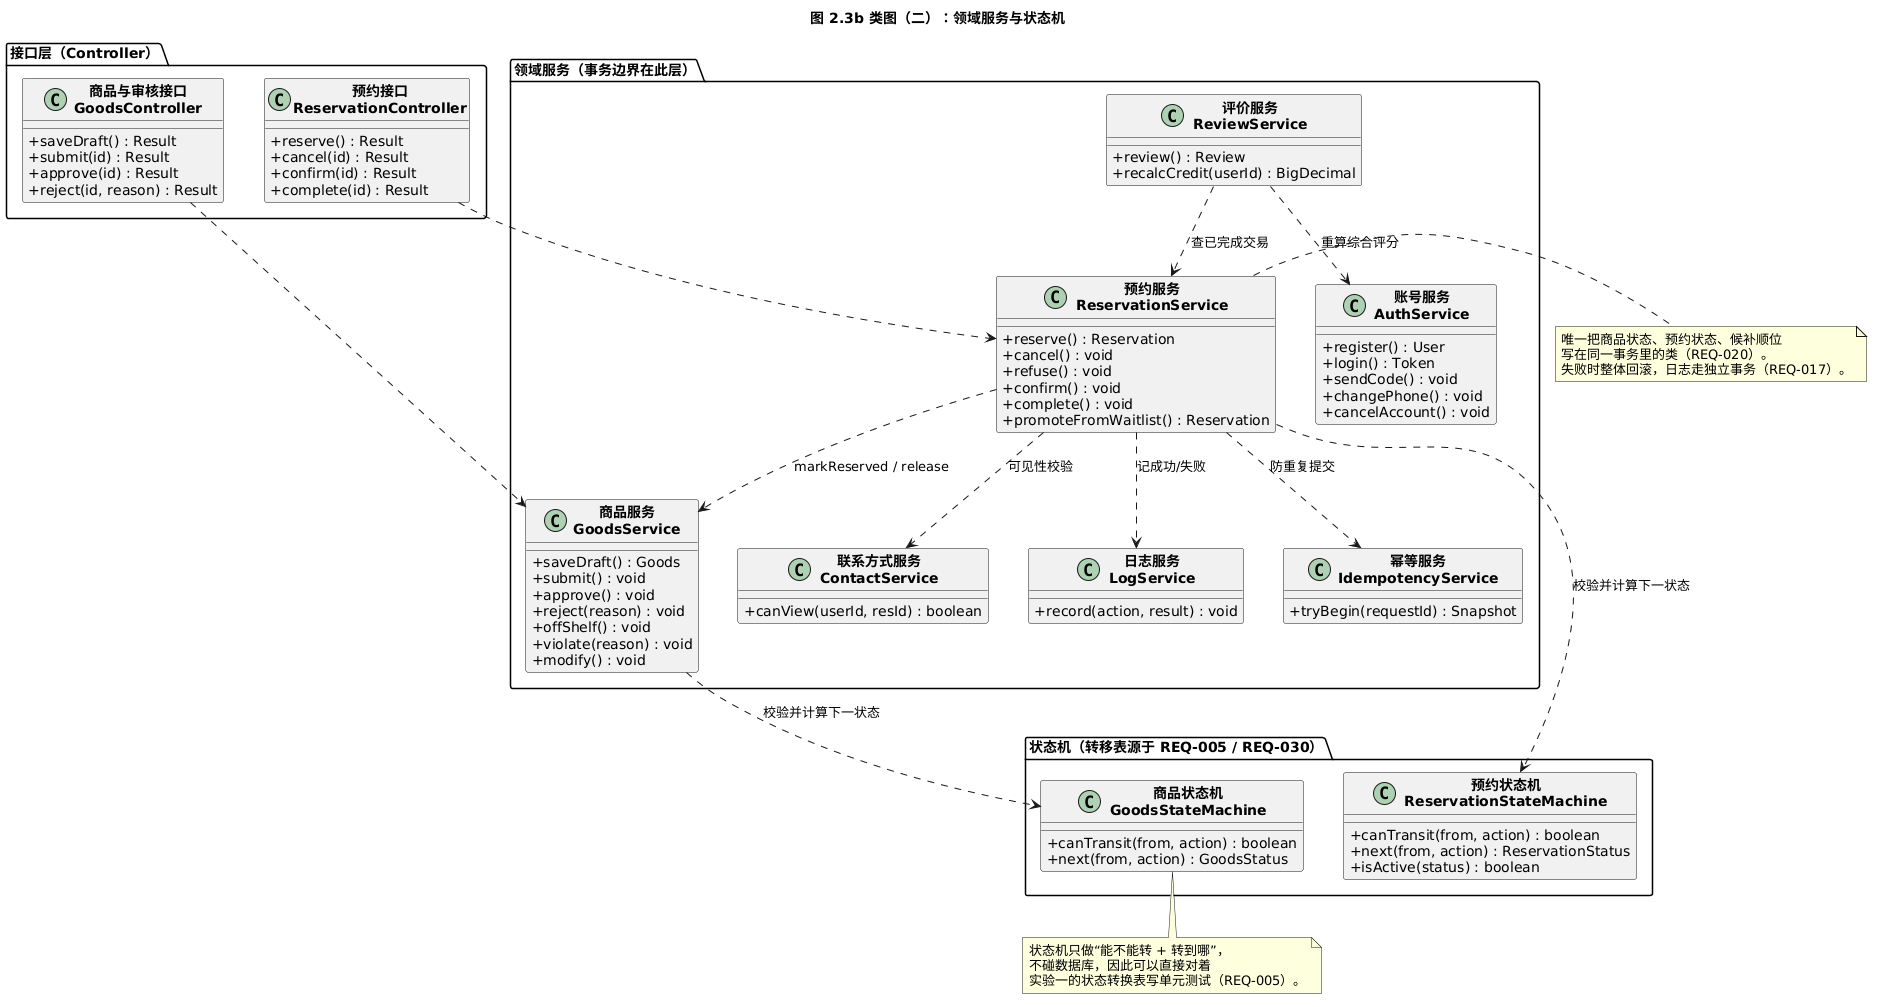
\includegraphics[width=\textwidth]{UML类图-服务.png}
\caption{领域服务与状态机类图}\label{fig:class2}
\end{figure}
\todo{说明状态机的职责边界，以及为什么事务边界放在 service 层。}

\subsection{状态图：商品与预约的状态机}
\begin{figure}[H]
\centering
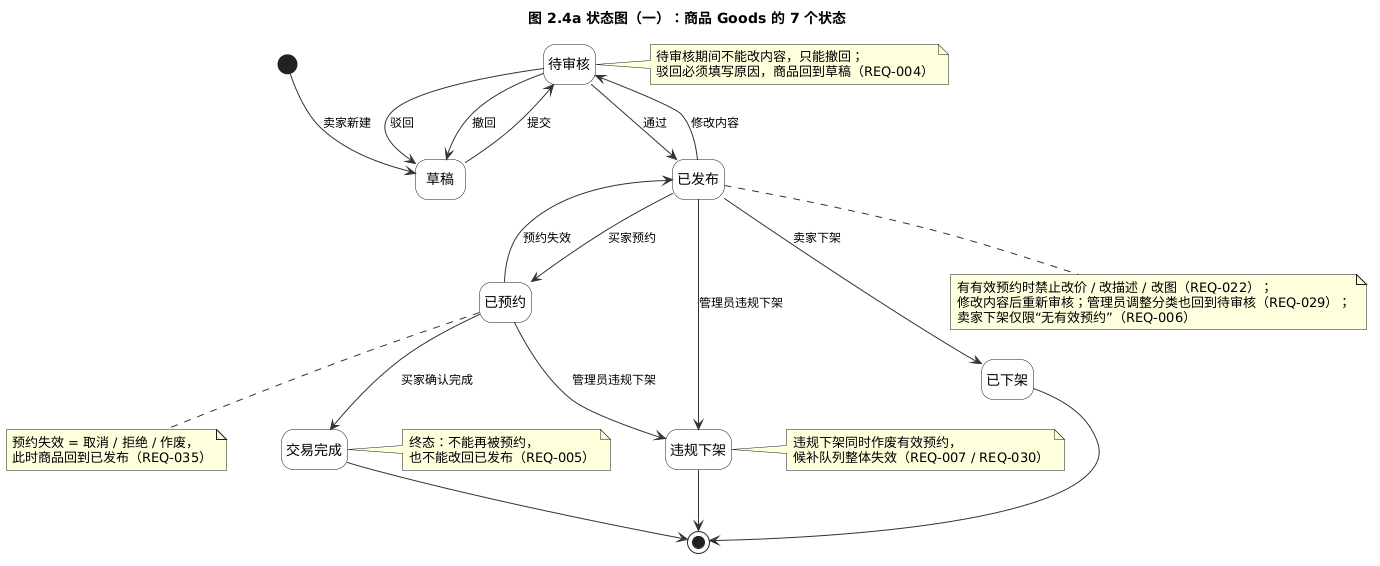
\includegraphics[width=\textwidth]{UML状态图-商品.png}
\caption{商品状态图}\label{fig:state-goods}
\end{figure}
\begin{figure}[H]
\centering
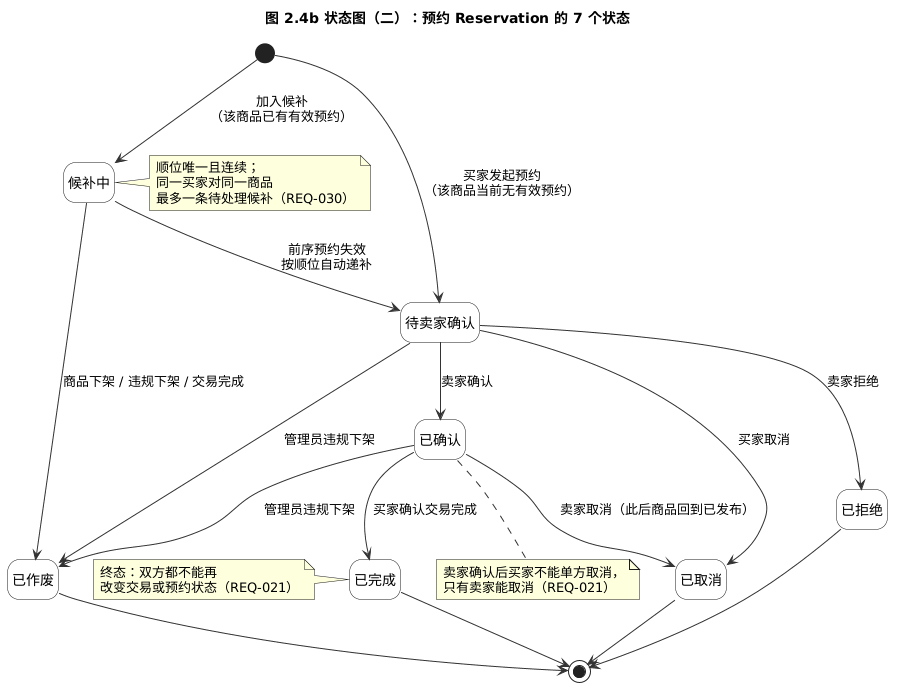
\includegraphics[width=0.82\textwidth]{UML状态图-预约.png}
\caption{预约状态图}\label{fig:state-res}
\end{figure}
\todo{把两张状态图与实验一的允许/禁止转换表对齐，指出哪几条转换是"必须拒绝"的，以及拒绝后状态如何保持不变。}

\subsection{用例图：角色与权限边界}
\begin{figure}[H]
\centering
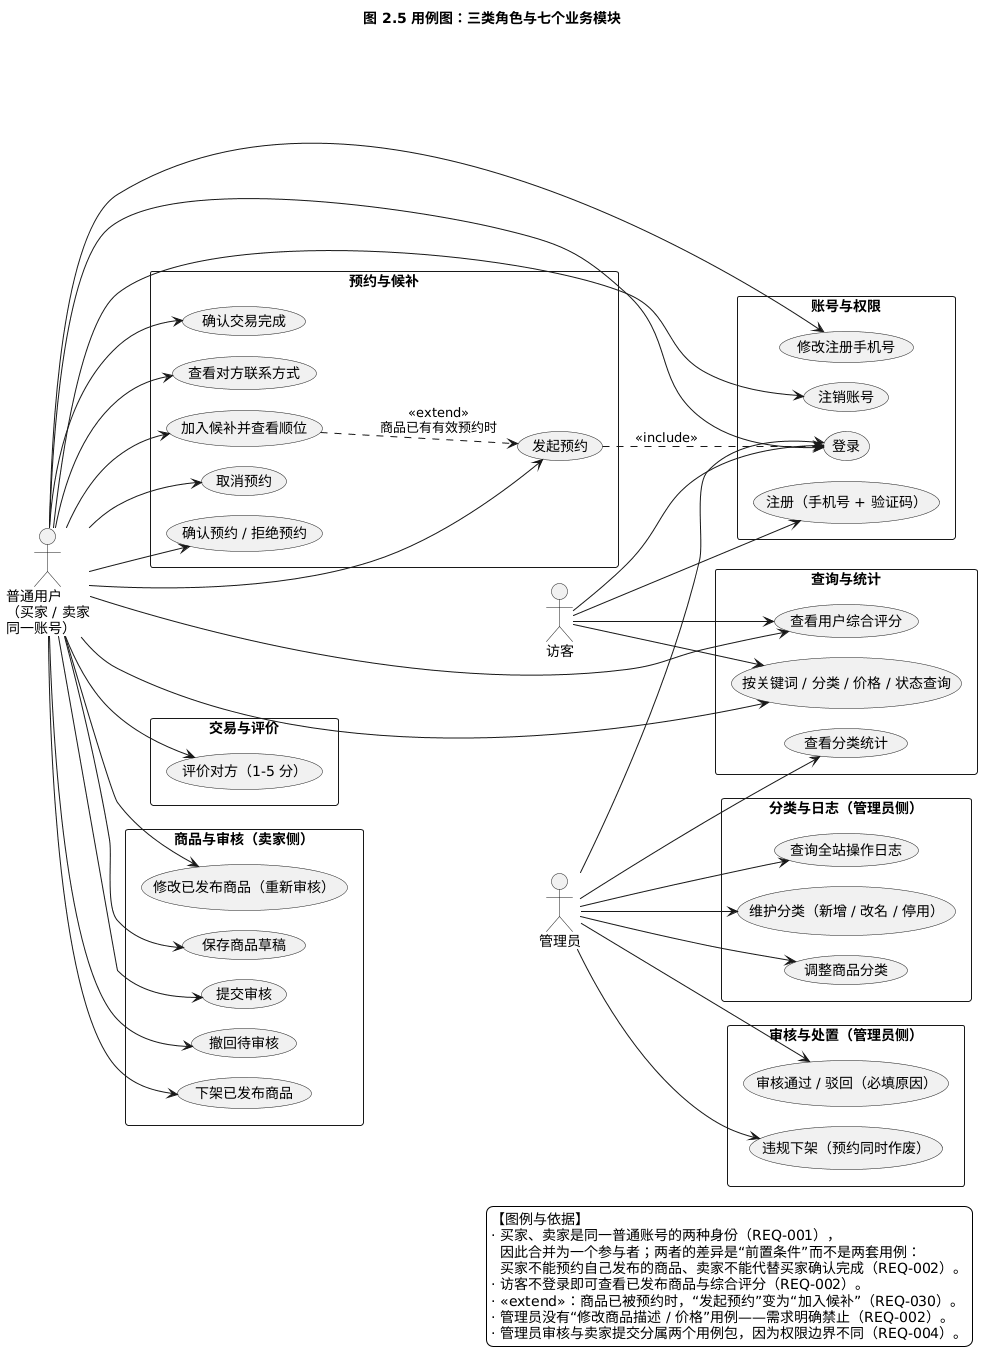
\includegraphics[width=0.78\textwidth]{UML用例图.png}
\caption{系统用例图}\label{fig:usecase}
\end{figure}
\todo{说明三类角色的边界、为什么买家与卖家合并为一个参与者、\texttt{include/extend} 的含义。}

\subsection{活动图：主流程与回退分支}
\begin{figure}[H]
\centering
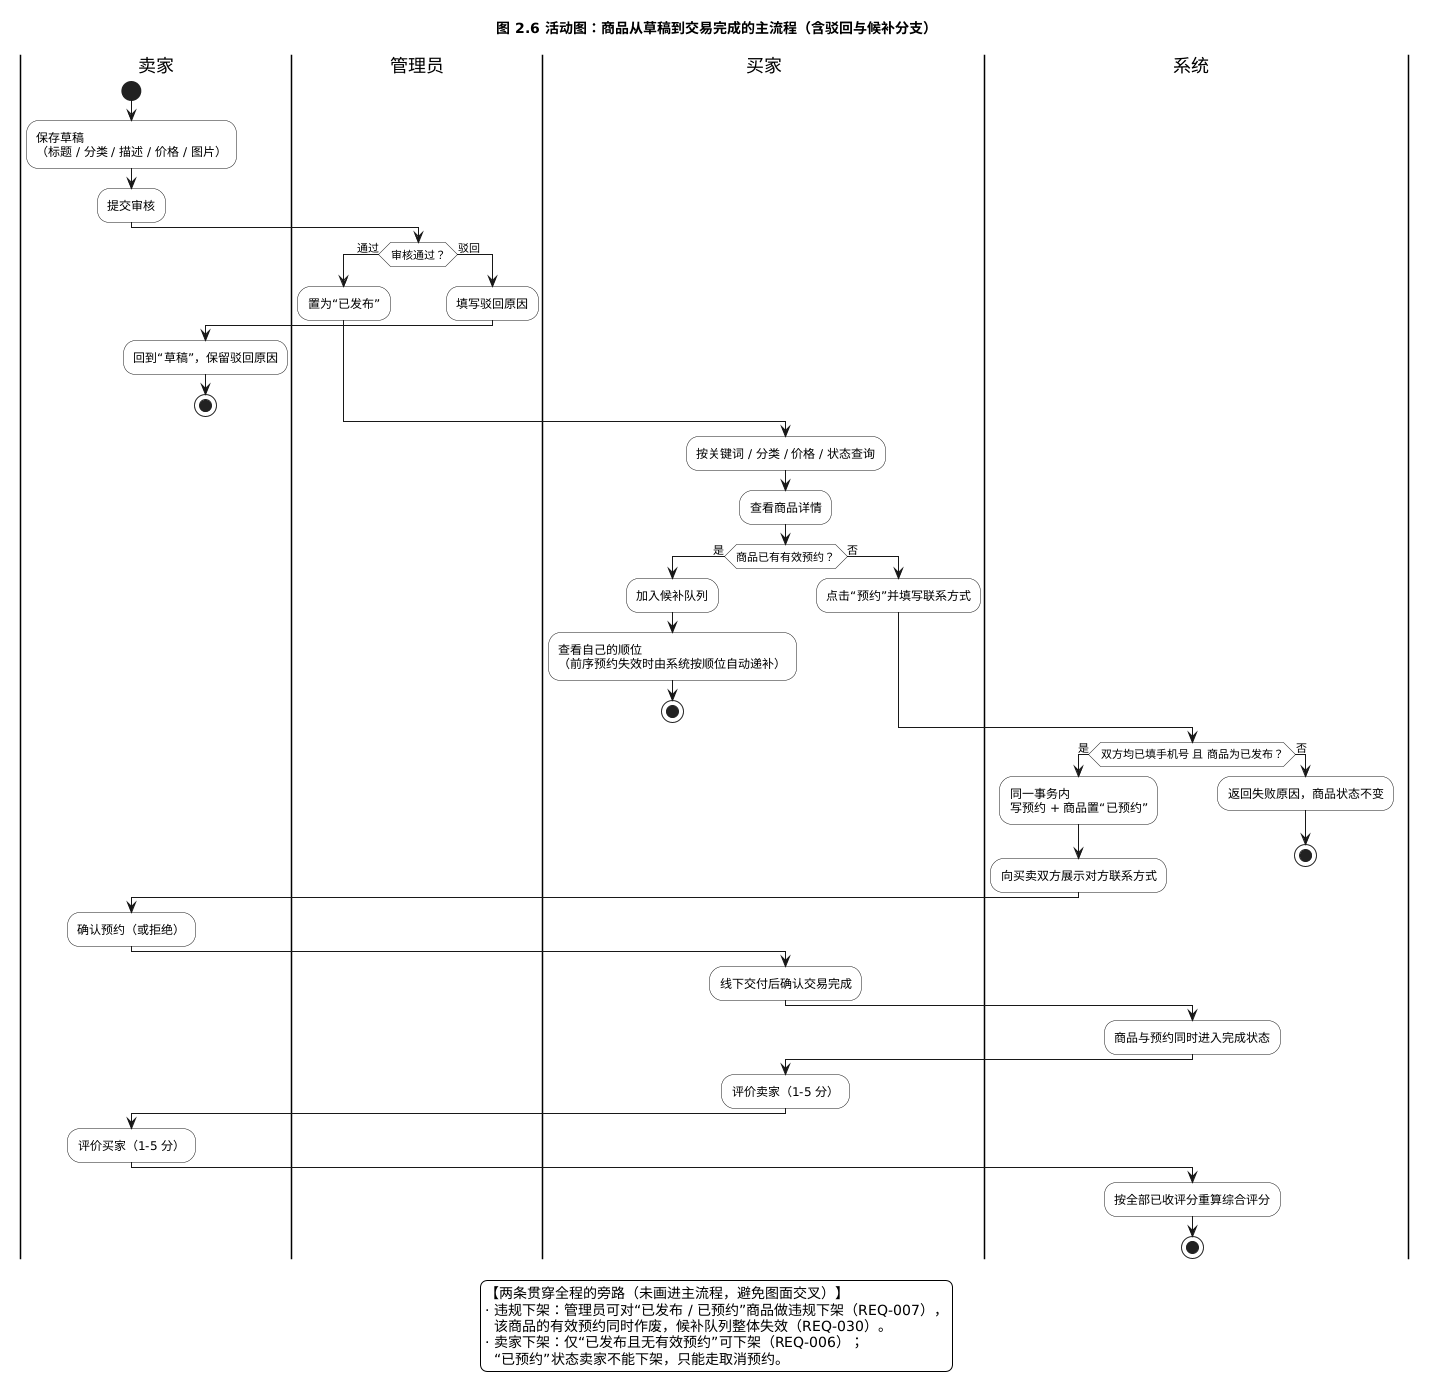
\includegraphics[width=0.96\textwidth]{UML活动图.png}
\caption{商品从草稿到交易完成的活动图}\label{fig:activity}
\end{figure}
\todo{讲主流程、驳回分支、候补分支，以及泳道划分的理由。}

\subsection{时序图：预约与取消递补}
\begin{figure}[H]
\centering
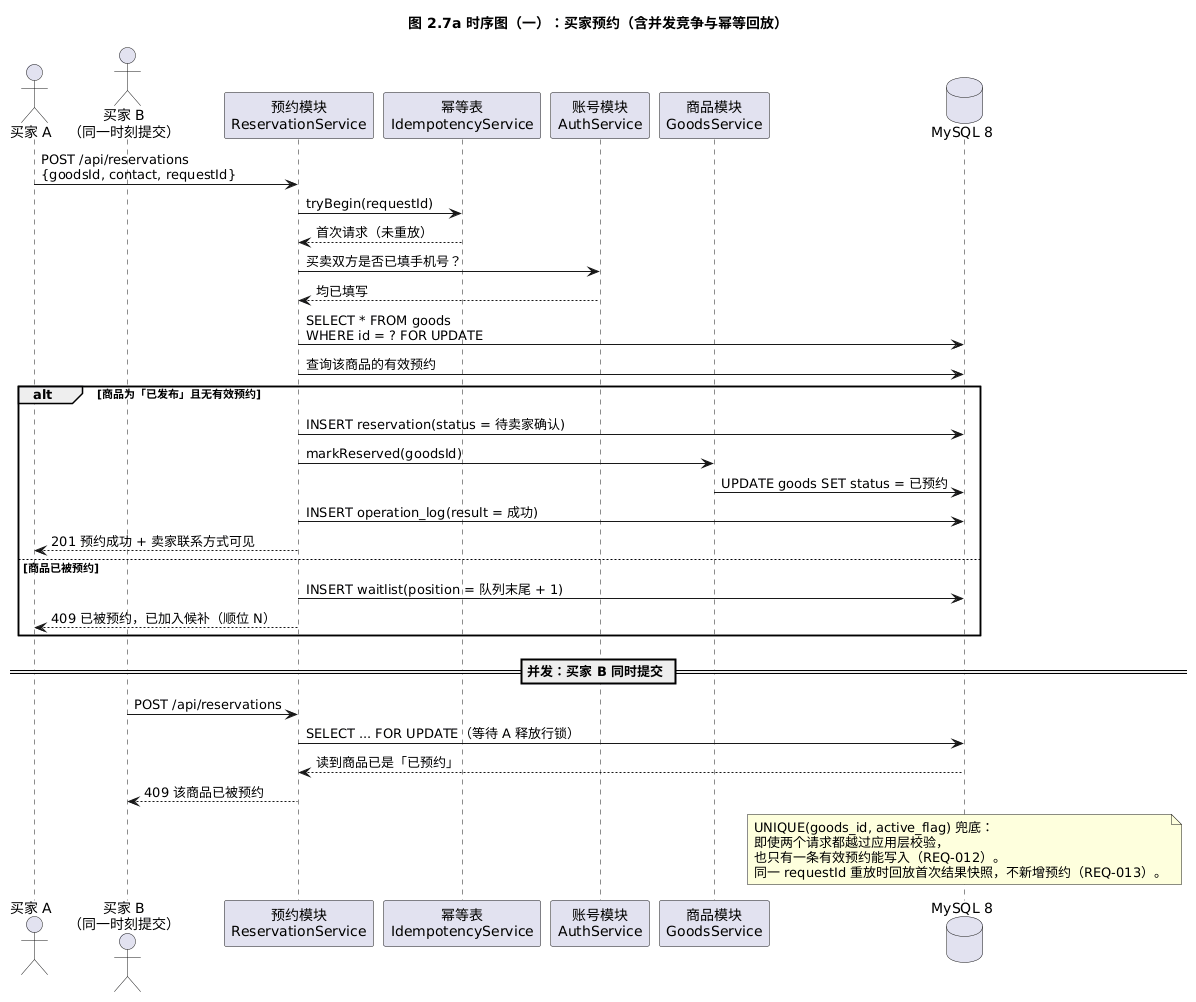
\includegraphics[width=0.82\textwidth]{UML时序图-预约与并发.png}
\caption{买家预约（含并发竞争与幂等回放）}\label{fig:seq1}
\end{figure}
\begin{figure}[H]
\centering
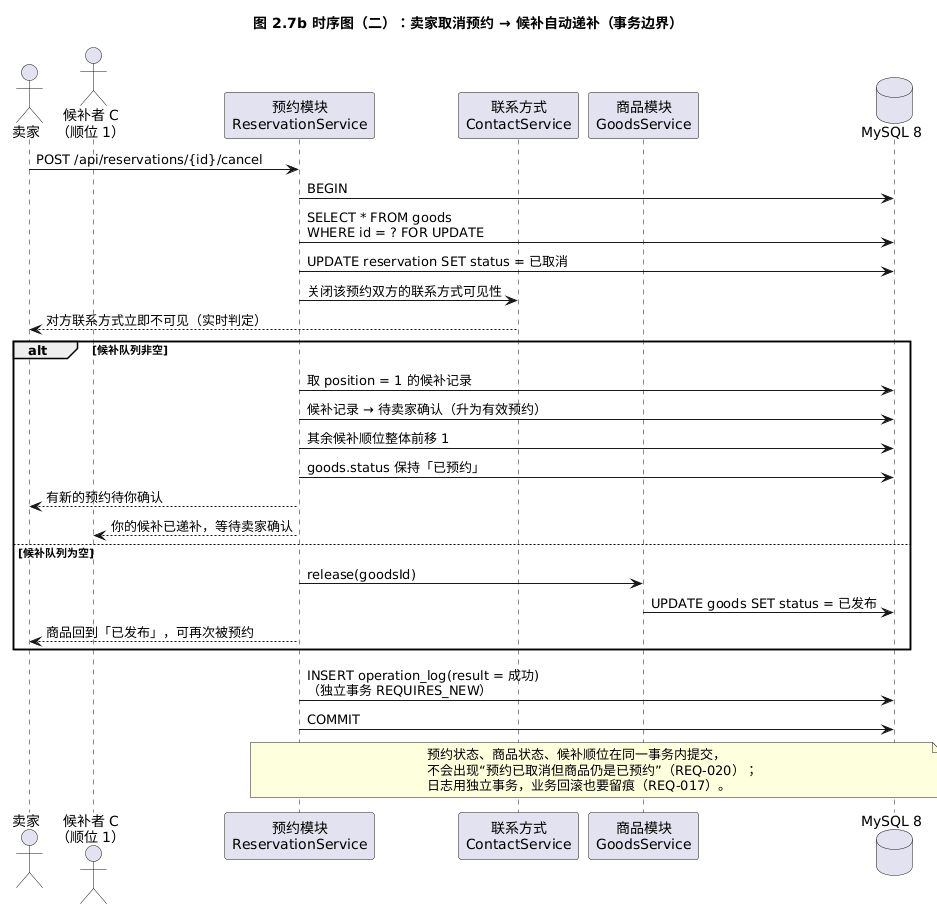
\includegraphics[width=0.80\textwidth]{UML时序图-取消与递补.png}
\caption{卖家取消预约与候补自动递补}\label{fig:seq2}
\end{figure}
\todo{结合两张时序图讲并发下"只有一人成功"如何保证、幂等如何回放、取消后商品如何回退与递补。}

\subsection{部署图}
\begin{figure}[H]
\centering
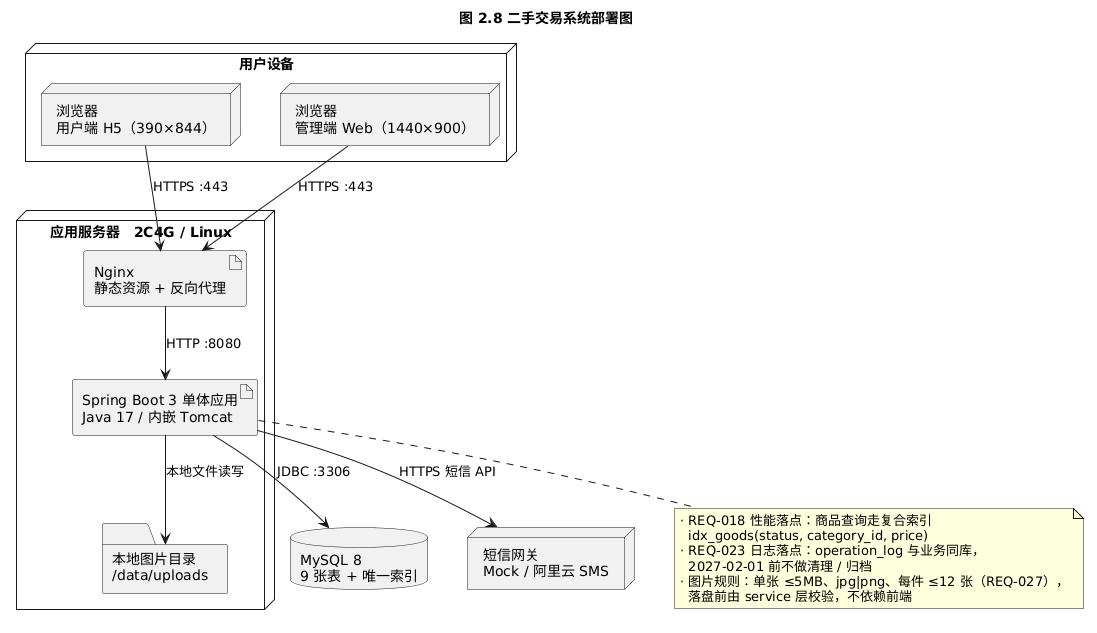
\includegraphics[width=0.86\textwidth]{UML部署图.png}
\caption{系统部署图}\label{fig:deploy}
\end{figure}
\todo{说明各节点的职责，以及性能（REQ-018）与日志保留（REQ-023）落在哪个节点。}

%=====================================================================
\section{各功能模块的 UI 界面及功能描述}

\subsection{设计规范}
\todo{写画幅（用户端 H5 390×844、管理端 1440×900）、色板、字号、组件规格；
本项目主张"用户端移动优先、管理端表格优先"的两端设计。}

% 两屏并排：\uipair{左图}{左标题}{label}{右图}{右标题}
\newcommand{\uipair}[5]{%
  \begin{figure}[H]\centering
  \begin{subfigure}[t]{0.48\textwidth}\centering
    \includegraphics[width=\textwidth]{#1}\caption{#2}
  \end{subfigure}\hfill
  \begin{subfigure}[t]{0.48\textwidth}\centering
    \includegraphics[width=\textwidth]{#4}\caption{#5}
  \end{subfigure}
  \caption{#2 与 #5}\label{#3}
  \end{figure}}

\subsection{账号与权限：01 登录注册、02 个人中心}
\uipair{01-登录注册.png}{登录注册}{fig:ui01}{02-个人中心.png}{个人中心}
\todo{相关模块 / 功能描述 / 对应需求（REQ-001、019、031、032、033）。下同。}

\subsection{查询与统计：03 首页商品列表}
\begin{figure}[H]\centering
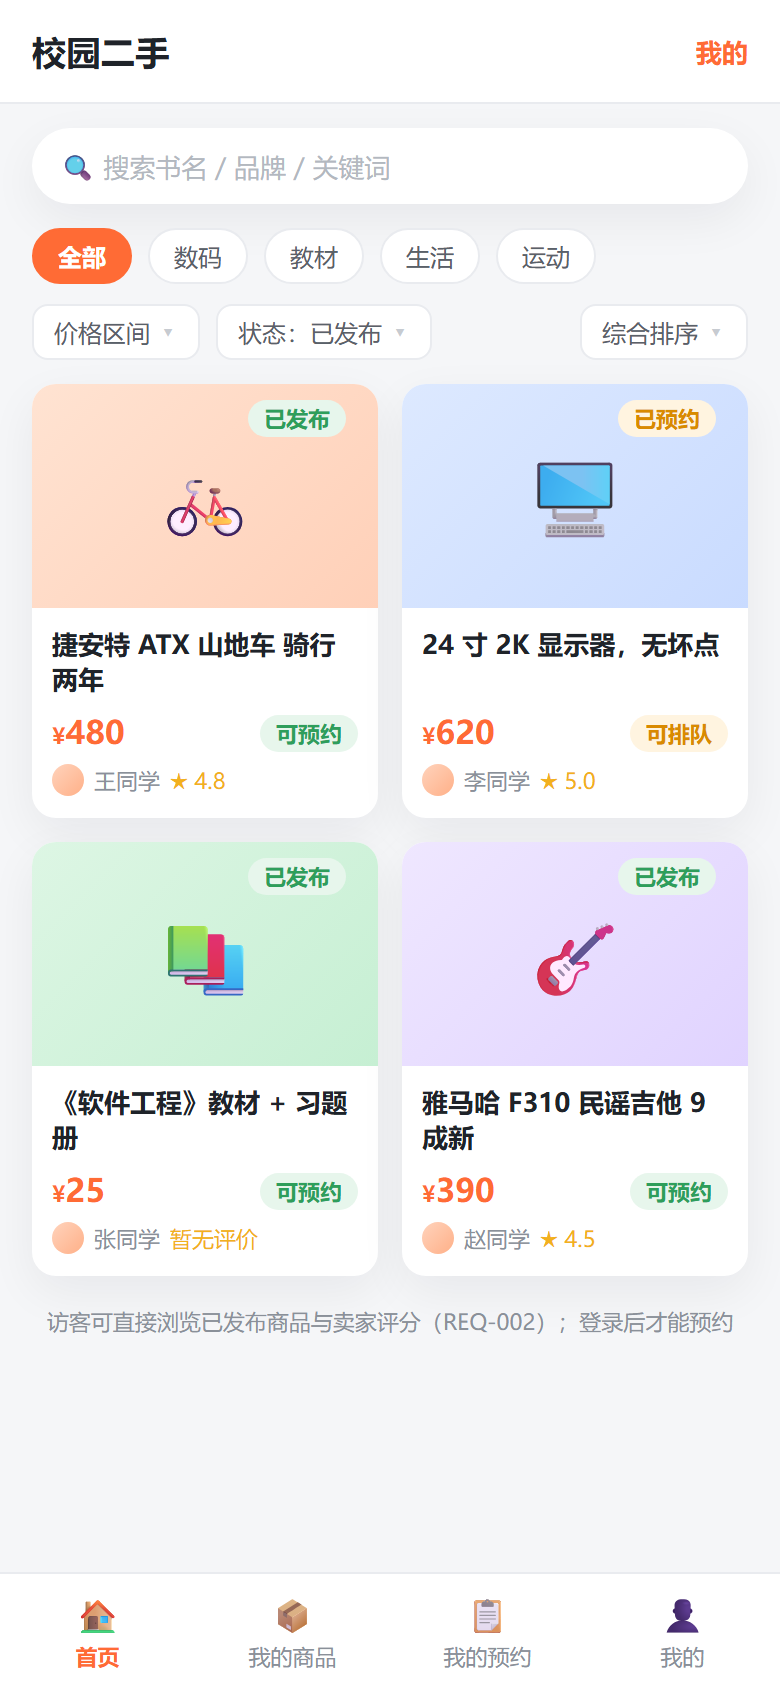
\includegraphics[width=0.42\textwidth]{03-首页商品列表.png}
\caption{首页商品列表}\label{fig:ui03}
\end{figure}
\todo{说明搜索、分类、价格与状态筛选；访客可见范围（REQ-008）。}

\subsection{商品与审核 + 预约：04 商品详情、05 预约确认}
\uipair{04-商品详情.png}{商品详情}{fig:ui04}{05-预约确认.png}{预约确认}
\todo{详情页说明联系方式可见性（REQ-024）；预约页说明 5 步 / 4 次操作 / 1 个必填项（REQ-034）。}

\subsection{预约与候补：06 我的预约（买家）、07 我的预约（卖家）}
\uipair{06-我的预约-买家.png}{我的预约（买家）}{fig:ui06}{07-我的预约-卖家.png}{我的预约（卖家）}
\todo{说明取消/拒绝/确认的入口与禁用条件、候补顺位展示（REQ-010、011、021、030）。}

\subsection{商品与审核：08 卖家商品管理、09 商品编辑}
\uipair{08-卖家商品管理.png}{卖家商品管理}{fig:ui08}{09-商品编辑.png}{商品编辑（含价格校验）}
\todo{说明 7 个状态下的可用操作、驳回原因展示、价格与图片校验（REQ-004、006、014、022、027）。}

\subsection{管理端：10 审核台、11 分类管理}
\begin{figure}[H]\centering
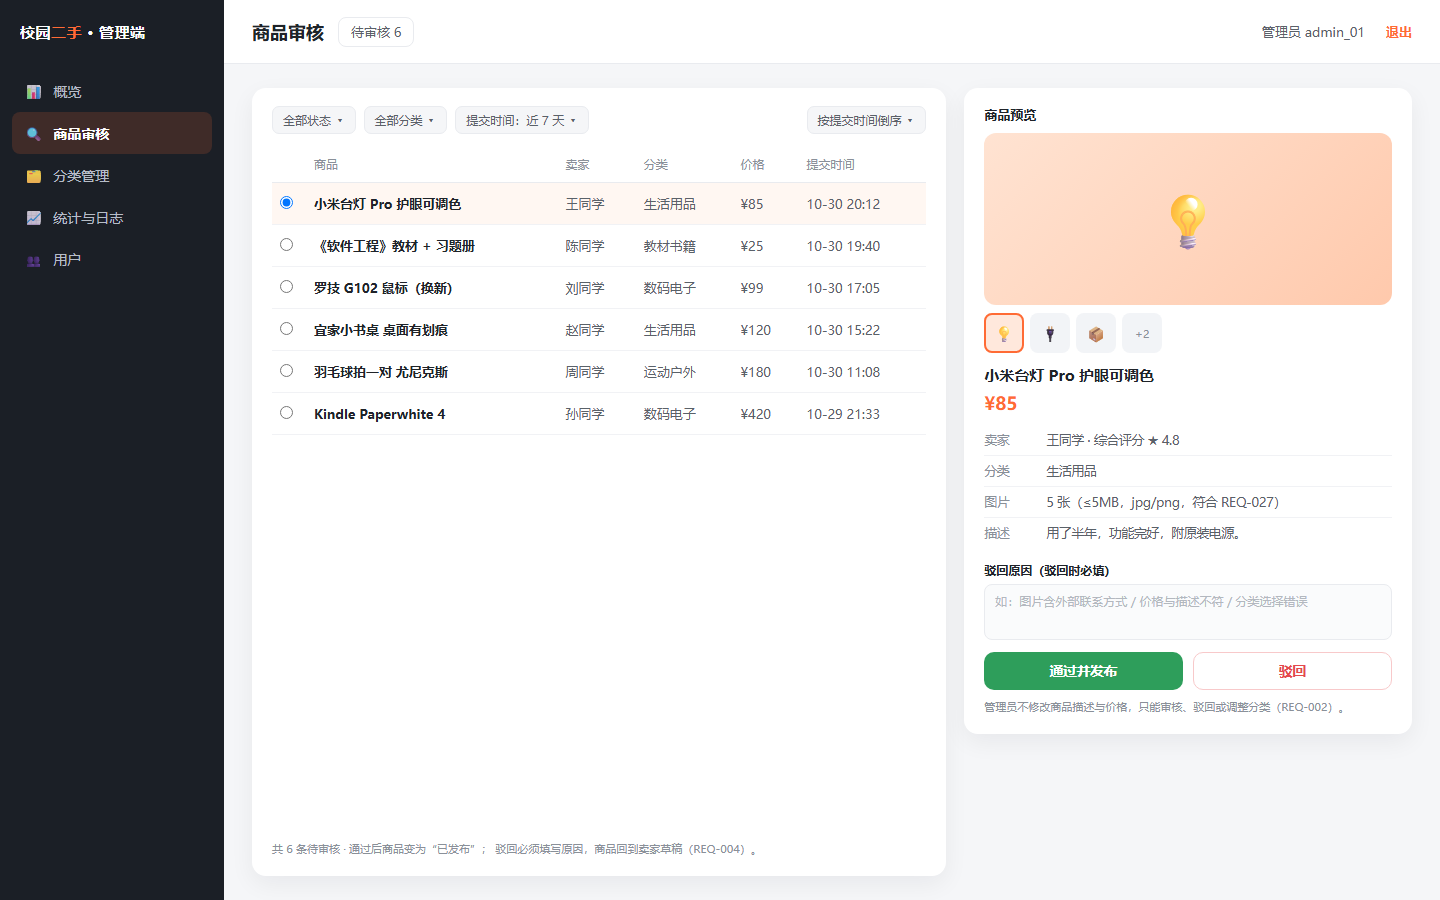
\includegraphics[width=\textwidth]{10-管理员审核台.png}
\caption{管理员审核台}\label{fig:ui10}
\end{figure}
\begin{figure}[H]\centering
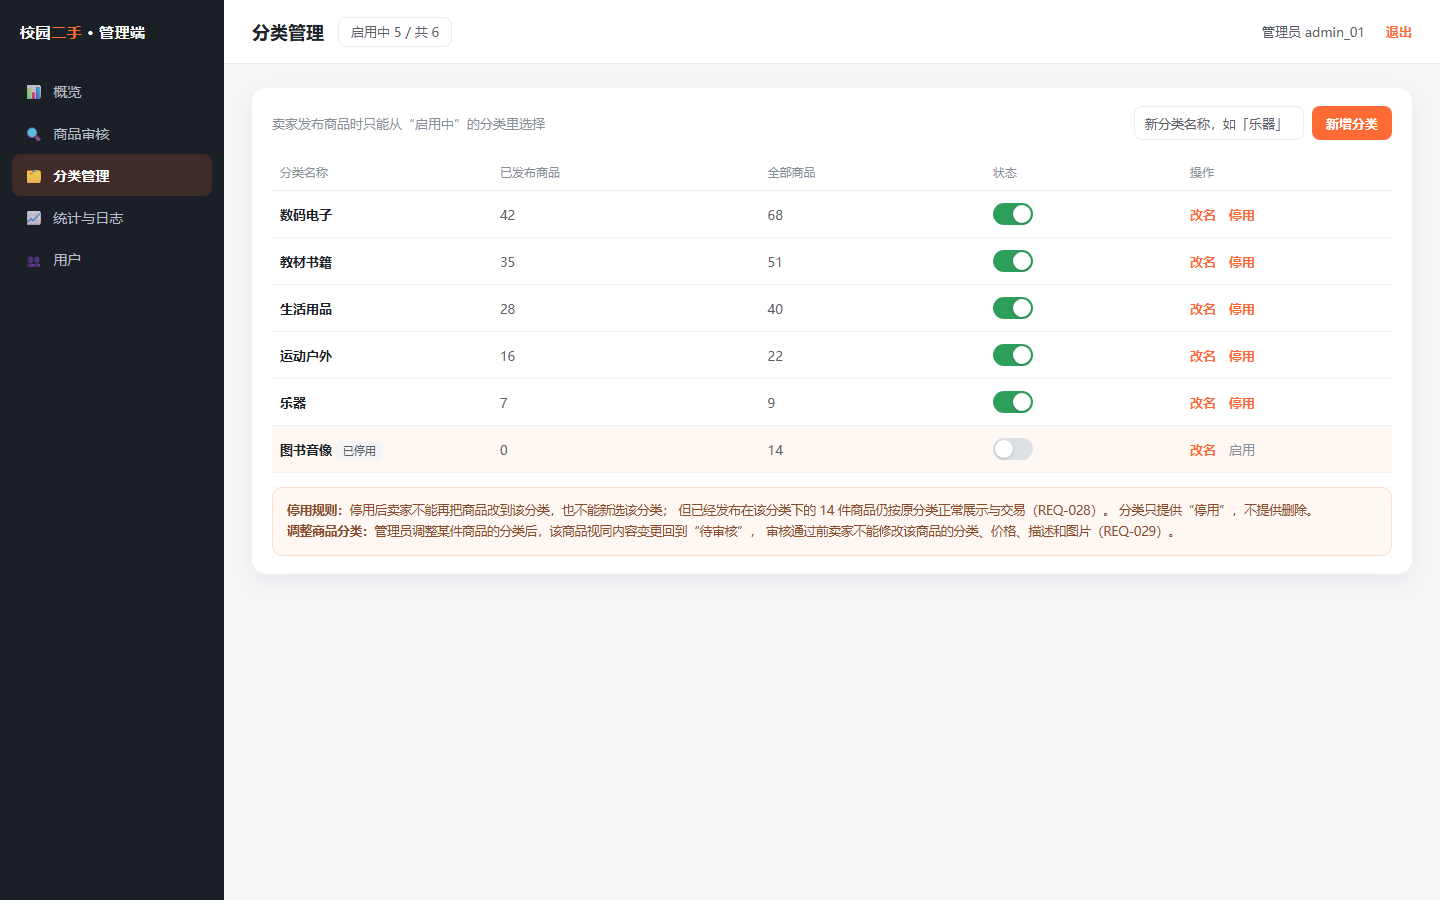
\includegraphics[width=\textwidth]{11-管理员分类管理.png}
\caption{管理员分类管理}\label{fig:ui11}
\end{figure}
\todo{说明审核与驳回、分类增改停用与"改分类回待审核"的联动（REQ-004、007、028、029）。}

\subsection{管理端：12 统计与日志}
\begin{figure}[H]\centering
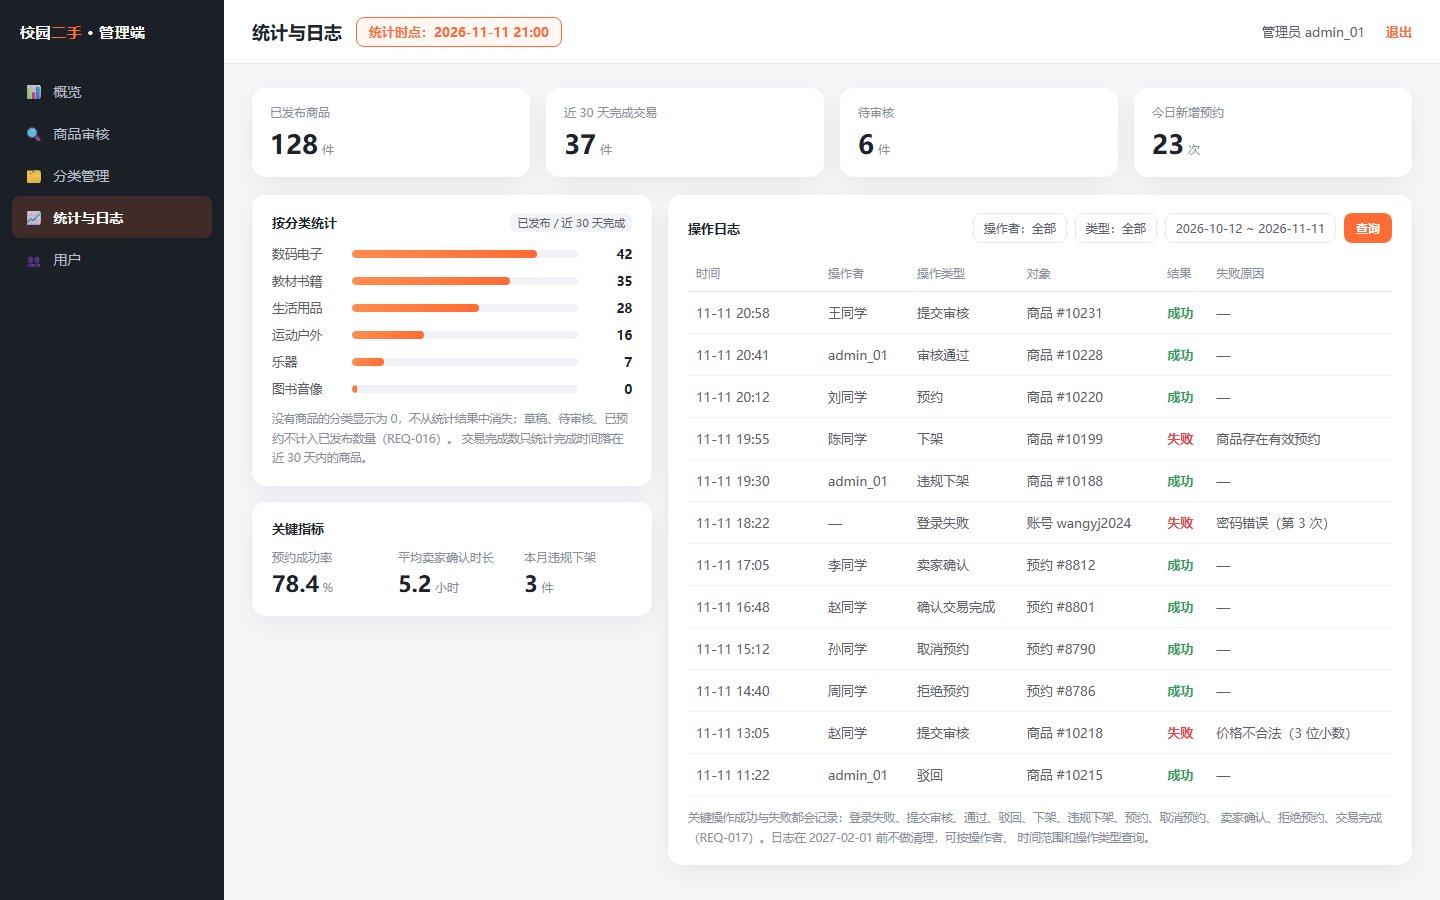
\includegraphics[width=\textwidth]{12-管理员统计与日志.png}
\caption{统计与操作日志}\label{fig:ui12}
\end{figure}
\todo{说明统计口径与日志字段、查询条件（REQ-016、017、023）。}

\subsection{交易与评价：13 交易完成与评价}
\begin{figure}[H]\centering
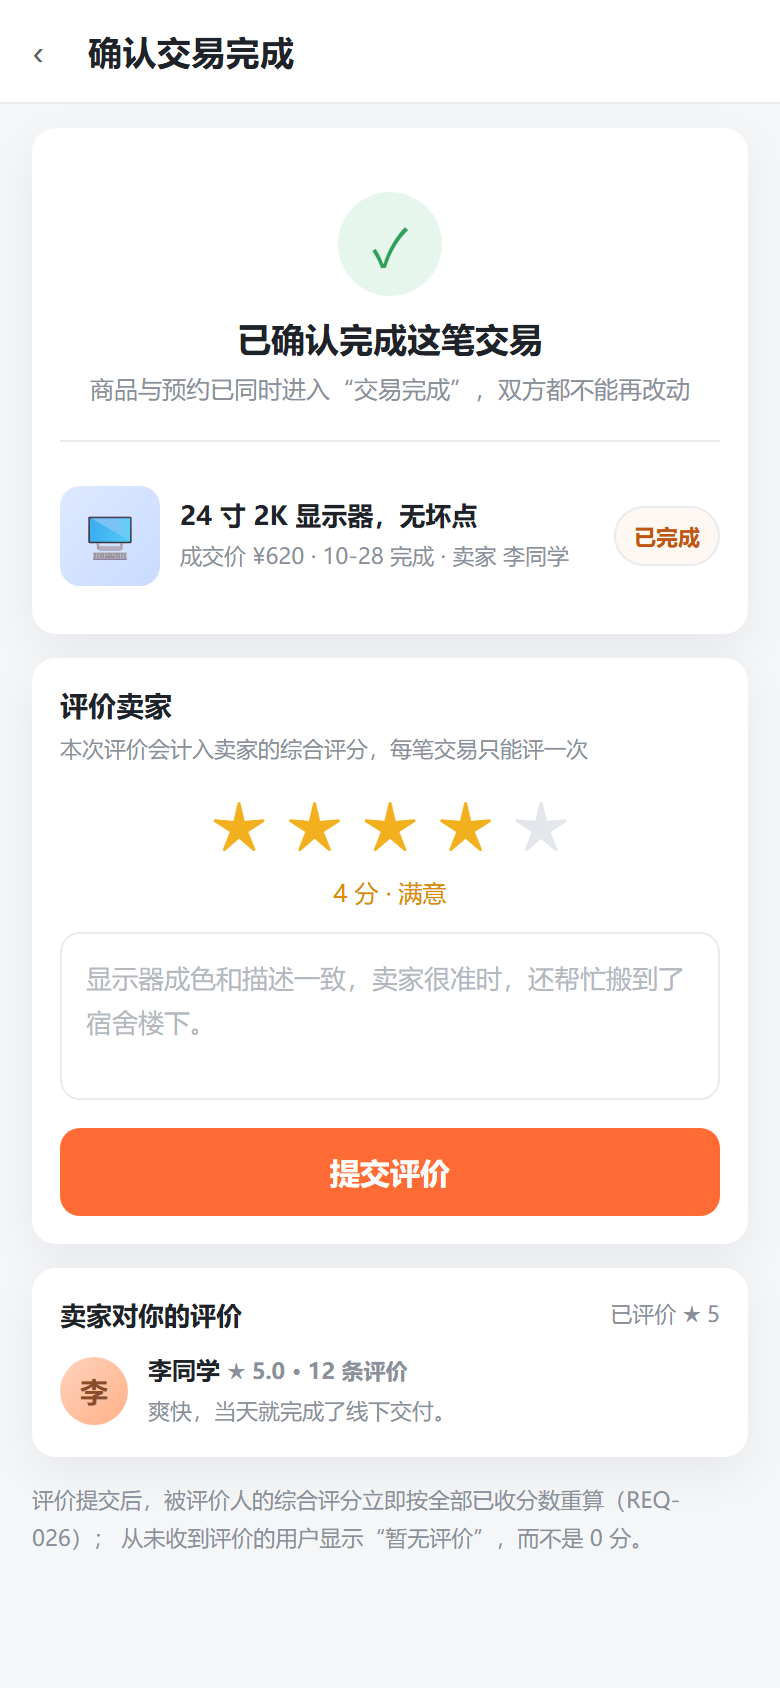
\includegraphics[width=0.42\textwidth]{13-交易完成与评价.png}
\caption{交易完成与评价}\label{fig:ui13}
\end{figure}
\todo{说明一次性评价约束与综合评分的"暂无评价"口径（REQ-025、026）。}

%=====================================================================
\section{大模型辅助设计的使用记录}

\subsection{记录一：模块划分方案的取舍}
\todo{使用场景 / 生成结果（截图可放附录）/ 优缺点分析 / 修改优化后的结果。}

\subsection{记录二：PlantUML 代码生成}
\todo{同上。建议写清模型生成的类图漏掉了什么、你补了什么（例如唯一有效预约的表达）。}

\subsection{记录三：界面控件与交互方案}
\todo{同上。建议写清模型给的建议哪里超出了需求边界、你如何删减。}

\subsection{记录四：设计评审与缺陷发现}
\todo{同上。建议写清模型提出的并发/一致性问题，以及你采纳后改到哪张图里。}

\subsection{大模型可以怎样辅助软件设计}
\todo{从自己的体验出发总结：适合发散与样板、不适合代替判断与约束校验。}

%=====================================================================
\section{总结与遗留问题}

\todo{设计取舍的回顾、与实验三实现的衔接、尚未解决的 TODO。}

\appendix
\section{数据库表结构}

\todo{用一段话说明：9 张表由类图的 9 个实体直接映射，两个唯一索引分别承担“唯一有效预约”与“幂等”两条硬约束。}

{\footnotesize
\begin{longtable}{p{2.9cm}p{4.8cm}p{5.0cm}p{2.1cm}}
\toprule
表 & 关键字段 & 唯一索引 / 约束 & 对应需求 \\
\midrule
\endhead
\texttt{user} & id, username, password\_hash, phone, role, status, fail\_count, lock\_until, cancelled\_at & uk\_user\_username(username)；uk\_user\_phone(phone) & 001 002 019 031 032 033 \\
\texttt{sms\_code} & phone, code, purpose, expire\_at, used\_at & uk\_sms(phone, purpose, code) & 031 032 \\
\texttt{category} & id, name, enabled, sort\_no & uk\_category\_name(name) & 028 029 \\
\texttt{goods} & id, seller\_id, category\_id, title, description, price, status, reject\_reason, violation\_reason, published\_at, completed\_at & idx\_goods\_query(status, category\_id, price)；idx\_goods\_seller(seller\_id, status) & 003--008 014 016 018 022 027 \\
\texttt{goods\_image} & id, goods\_id, url, size\_bytes, content\_type, sort\_no & fk\_goods\_image(goods\_id, sort\_no)；≤12 张由 service 校验 & 027 \\
\texttt{reservation} & id, goods\_id, buyer\_id, status, \textbf{active\_flag}\newline（生成列）, extra\_contact, request\_id, created\_at, confirmed\_at, completed\_at & \textbf{uk\_active\_reservation}\newline (goods\_id, active\_flag)；\newline uk\_reservation\_request\newline (request\_id) & 009--013\newline 020 021\newline 024 030\newline 035 \\
\texttt{waitlist}\allowbreak\texttt{\_entry} & id, goods\_id, buyer\_id, position, created\_at & uk\_waitlist\_pos(goods\_id, position)；uk\_waitlist\_buyer(goods\_id, buyer\_id) & 030 \\
\texttt{review} & id, reservation\_id, reviewer\_id, reviewee\_id, score, comment, created\_at & uk\_review(reservation\_id, reviewer\_id) & 025 026 \\
\texttt{operation\_log} & id, operator\_id, action, target\_type, target\_id, result, fail\_reason, created\_at & idx\_log\_query(operator\_id, action, created\_at) & 017 023 \\
\bottomrule
\end{longtable}
}

\noindent 其中 \texttt{reservation.active\_flag} 由 \texttt{status} 生成：状态属于“待卖家确认 / 已确认”时取 1，其余取 NULL；
配合 \texttt{UNIQUE(goods\_id, active\_flag)}，同一商品在任一时刻最多只能写入一条有效预约——这是 REQ-012
“并发下只有一人成功”的最后一道防线，应用层的 \texttt{SELECT ... FOR UPDATE} 只是提前给出可读的失败提示。

\section{需求—模块—界面追溯表}

\todo{用一段话说明：35 条需求逐条落到模块与界面/图形，保证“没有需求没被设计覆盖”。}

{\footnotesize
\begin{longtable}{p{1.55cm}p{4.1cm}p{0.8cm}p{3.85cm}p{4.1cm}}
\toprule
编号 & 需求 & 模块 & 界面 / 图形 & 落点说明 \\
\midrule
\endhead
REQ-001 & 普通用户注册与登录 & M1 & 01 登录注册 & 手机号 + 验证码注册 \\
REQ-002 & 三类角色的操作权限 & M1 & 全站 & 角色拦截器统一校验 \\
REQ-003 & 保存商品草稿 & M2 & 09 商品编辑 & 草稿仅本人可见 \\
REQ-004 & 提交审核、通过、驳回、撤回 & M2 & 08 卖家管理、10 审核台 & 驳回必填原因 \\
REQ-005 & 商品状态与允许的转换 & M2 & 图 5 商品状态图 & 状态机转移表 \\
REQ-006 & 卖家下架已发布商品 & M2 & 08 卖家管理 & 下架按钮的禁用条件 \\
REQ-007 & 管理员违规下架 & M2 & 10 审核台 & 违规下架并作废预约 \\
REQ-008 & 按关键词 / 分类 / 价格 / 状态查询 & M4 & 03 首页列表 & 四条件组合与可见范围 \\
REQ-009 & 买家发起预约 & M5 & 04 详情、05 预约确认 & 双方联系方式齐备才可预约 \\
REQ-010 & 确认前取消或拒绝预约 & M5 & 06 买家预约 & 取消 / 拒绝无需对方同意 \\
REQ-011 & 卖家确认与买家确认完成 & M5 & 06、07、13 & 确认 → 完成两步走 \\
REQ-012 & 同一商品只有一条有效预约 & M5 & 05 预约确认 & 唯一索引 + 行锁 \\
REQ-013 & 重复提交与旧页面操作 & M5 & 05 预约确认 & requestId 幂等回放 \\
REQ-014 & 非法价格拒绝保存 & M7 & 09 商品编辑 & 错误态与提示文案 \\
REQ-015 & 用户、商品、预约数据一致 & M7 & 附录 A & 唯一索引与外键 \\
REQ-016 & 按分类与完成情况统计 & M4 & 12 统计与日志 & 无商品分类显示 0 \\
REQ-017 & 关键操作日志记录与查询 & M7 & 12 统计与日志 & 成功与失败都记 \\
REQ-018 & 商品查询响应时间 & M4 & 03 首页列表 & 复合索引 idx\_goods\_query \\
REQ-019 & 密码摘要与连续失败锁定 & M1 & 01 登录注册 & 5 次错误锁 10 分钟 \\
REQ-020 & 预约与状态变更的原子性 & M7 & 图 10 时序图（一） & 同一事务提交 \\
REQ-021 & 确认后取消与完成的锁定 & M5 & 06 买家预约 & 确认后仅卖家可取消 \\
REQ-022 & 已发布商品修改后重新审核 & M2 & 08、09 & 有预约时禁止修改 \\
REQ-023 & 操作日志保留期限 & M7 & 12 统计与日志 & 2027-02-01 前不清理 \\
REQ-024 & 预约成功后的联系方式展示 & M5 & 04、06、07 & 可见性实时判定 \\
REQ-025 & 交易完成后双方互评 & M6 & 13 交易完成与评价 & 每笔每方一次 \\
REQ-026 & 用户综合评分展示 & M6 & 03、04、13 & 无评价显示“暂无评价” \\
REQ-027 & 图片数量、大小与格式 & M2 & 09 商品编辑 & 12 张 / 5MB / jpg 或 png \\
REQ-028 & 管理员维护商品分类 & M3 & 11 分类管理 & 只能停用不能删除 \\
REQ-029 & 调整分类后的审核与锁定 & M3 & 11 分类管理 & 改分类视同内容变更 \\
REQ-030 & 候补队列与自动递补 & M5 & 06、07 & 顺位唯一且连续 \\
REQ-031 & 手机号注册与验证 & M1 & 01 登录注册 & 一号一账号 \\
REQ-032 & 修改注册手机号 & M1 & 02 个人中心 & 新旧号双验证 \\
REQ-033 & 账号注销与数据可见性 & M1 & 02 个人中心 & 有未完成交易时拒绝 \\
REQ-034 & 预约主流程步骤数与易用性 & M5 & 05 预约确认 & 5 步 / 4 次操作 / 1 必填 \\
REQ-035 & 卖家取消后商品回到已发布 & M5 & 07 卖家预约 & 有候补时自动递补 \\
\bottomrule
\end{longtable}
}

\end{document}
